%\renewcommand{\theequation}{\theenumi}
%\begin{enumerate}[label=\arabic*.,ref=\thesubsection.\theenumi]
%\numberwithin{equation}{enumi}

\item Find the equation of the circle passing through \myvec{0\\0} and making intercepts a and b on the coordinate axes.
\\
\solution
Let 
\begin{align}
 \vec{A}=\myvec{a\\0} ,
 \vec{B}=\myvec{b\\0},
 \vec{C}=\myvec{0\\0}
\end{align}
Since the circle passes through $\myvec{0\\0}$, the equation of given circle is,
\begin{align}
    \vec{x^\top}\vec{x}+2\vec{u^\top}\vec{x}=0 \label{quadform/july/2/1/eq:0}
\end{align}

The general equation of circle is,
\begin{align}
\vec{x^\top}\vec{x}+2\vec{u^\top}\vec{x}+f=0 
\end{align}
% Given intercepts are $\myvec{a\\0}$ and $\myvec{0\\b}$ \\
% \begin{figure}[!h]
%          \centering
%          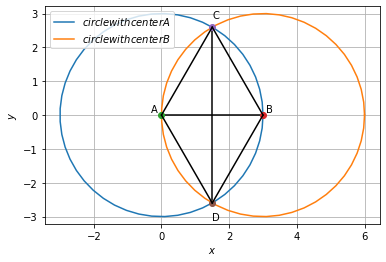
\includegraphics[width=\columnwidth]{figure3.png}
%          \caption{Plot of the required circle}
%          \label{quadform/july/2/1/Figure}
% \end{figure}\\
Substituting $ \vec{A},  \vec{B}$ in \eqref{quadform/july/2/1/eq:0},
\begin{align}
    \vec{A^\top}\vec{A}+2\vec{u^\top}\vec{A}=0 \label{quadform/july/2/1/eq:4}
    \\
    \vec{B^\top}\vec{B}+2\vec{u^\top}\vec{B}=0 \label{quadform/july/2/1/eq:5}
\end{align}
Simplifying \eqref{quadform/july/2/1/eq:4} and \eqref{quadform/july/2/1/eq:5}
\begin{align}
    \myvec{a & 0 \\ 0 & b}\vec{u}^\top= -\frac{1}{2}\myvec{a^2 \\ b^2}
\end{align}
\begin{align}
\implies \myvec{a & 0 & -a^2/2 \\ 0 & b & -b^2/2}
\\
\xleftrightarrow [R_1\leftarrow R_1/a]{R_2\leftarrow R_2/b}
\myvec{1 & 0 & -a/2 \\ 0& 1 & -b/2}
\end{align}
\begin{align}
    \implies \vec{u}=-\frac{1}{2}\myvec{a \\ b}
     \\
     \text{or, } \vec{x^\top}\vec{x}-\myvec{a \\ b }\vec{x}=0
\end{align}
upon substituting  in \eqref{quadform/july/2/1/eq:0}.
% \begin{align}
%     \vec{x^\top}\vec{x}+2\myvec{-a/2 \\ -b/2}\vec{x}=0 
% \end{align}
% \begin{align}
 
% \end{align}
% is the desired equation of the circle.
% Substituting, $a=6$ and $b=8$,the circle is plotted.
% Equation of given circle is,
% \begin{align}
%    \implies \vec{x^\top}\vec{x}-\myvec{6 \\ 8 }\vec{x}=0
% \end{align}
%
\item Find the equation of a circle with centre \myvec{2\\2} and passes through the point \myvec{4\\5}. 
\\
\solution
From the given information, the centre 

\begin{align}
    \vec{c} = \myvec{2\\2} \implies   \vec {u}= -\vec{c} = \myvec{-2\\-2 }
\end{align}

Using the general equation of a circle and substituting $\vec{x} = \myvec{4\\5}$,

\begin{align}
    \label{quadforms/july/2/2/eq:1}
    \begin{split}
\vec{x^\top}\vec{x}+2\vec{u^\top}\vec{x}+f&=0 
\\
\implies     \myvec{4 \ 5}\myvec{4\\5}+\myvec{-4 \ -4}\myvec{4\\5}+f&=0
\\
\implies f+\myvec{41}+\myvec{-36} &= 0 
\\
\text{or, }  f &= -5
    \end{split}
\end{align}
%
Hence , the equation of the circle is,
\begin{align}
    \vec{x^\top}\vec{x}+\myvec{-4 \ -4 }\vec{x}-5=0
\end{align}
%
The radius of the circle is then given by 
\begin{align}
r = \sqrt{\vec{u^\top}\vec{u}-f}
\implies r = \sqrt{13}
\end{align}
%
The above results are verified in Fig.     \ref{quadforms/july/2/2/Figure}


\begin{figure}[!h]
    \centering
    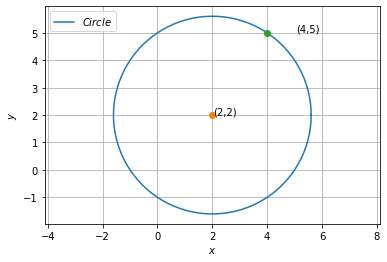
\includegraphics[width=\columnwidth]{solutions/july/2/2/Figures/Figure.png}
    \caption{Plot of the required circle}
    \label{quadforms/july/2/2/Figure}
\end{figure}

\item Find the locus of all the unit vectors in the xy-plane.
%
\item Find the points on the curve $\vec{x}^T\vec{x}-2\myvec{1 & 0}\vec{x} -3 =0$  at which the tangents are parallel to the x-axis.
%
\item  Find the area of the region in the first quadrant enclosed by x-axis, line $\myvec{1 & -\sqrt{3}}\vec{x} =0$ and the circle $\vec{x}^T\vec{x}=4$.
%
\item Find the area lying in the first quadrant and bounded by the circle $\vec{x}^T\vec{x}=4$ and the lines $x = 0$ and $x = 2$.
%
\item Find the area of the circle $4\vec{x}^T\vec{x}=9$.
\item  Find the area bounded by curves $\norm{\vec{x}-\myvec{1\\0}} = 1$ and $\norm{\vec{x}}=1$
\item Find the smaller area enclosed by the circle $\vec{x}^T\vec{x}=4$ and the line $\myvec{1 & 1}\vec{x} = 2$.
%\item The sum of the perimeter of a circle and square is $k$, where $k$ is some constant. Prove that the sum of their areas is least when the side of square is double the radius of the circle.
%\item A window is in the form of a rectangle surmounted by a semicircular opening. The total perimeter of the window is 10 m. Find the dimensions of the window to admit maximum light through the whole opening.
%
\item If 
$
\brak{x-a}^2+\brak{y-b}^2 = c^2,
$
for some $c > 0$, prove that 
\begin{align}
\frac{\brak{1+y_2}^\frac{3}{2}}{y_2}
\end{align}
%
is a constant independent of $a$ and $b$.
%
\item Form the differential equation of the family of circles touching the y-axis at origin.
\item Form the differential equation of the family of circles having centre on y-axis and radius 3 units.
\item Form the differntial equation of the fmaily of circles touching the x-axis at the origin.
%
\item Form the differential equation of the family of circles in the second quadrant and touching the coordinate axes.
\item Factorise $y^2 – 5y + 6$.
\item Find the zeroes of the quadratic polynomial $x^2+7x+10$ and verify the relationship between the zeroes and the coefficients.


\item Find a quadratic polynomial, the sum and product of whose zeroes are – 3 and 2, respectively.
\\
\solution
\begin{lemma}
The points of intersection of \textbf{Line} $L:\vec{x}=\vec{q}+\mu\vec{m}$ with \textbf{parabola}

\begin{align}
\vec{x^T}\vec{V}\vec{x}+2\vec{u^T}\vec{x}+f=0
\end{align}

is given by:
\begin{align}
\vec{x}_i = \vec{q}+\mu_i\vec{m}
\end{align}
%
where,
\begin{multline}
\mu_i = \frac{1}
{
\vec{m}^T\vec{V}\vec{m}
}
\lbrak{-\vec{m}^T\brak{\vec{V}\vec{q}+\vec{u}}}
\\
\pm
{\small
\rbrak{\sqrt{
\sbrak{
\vec{m}^T\brak{\vec{V}\vec{q}+\vec{u}}
}^2
-
\brak
{
\vec{q}^T\vec{V}\vec{q} + 2\vec{u}^T\vec{q} +f
}
\brak{\vec{m}^T\vec{V}\vec{m}}
}
}
}\label{2/37/quad}
\end{multline}
\end{lemma}
\begin{proof}
The points of intersection must satisfy the line and parabola equation.
Thus,
\begin{align}
\vec{\brak{\vec{q}+\mu\vec{m}}^T}\vec{V}\vec{\brak{\vec{q}+ \mu\vec{m}}}+2\vec{u^T}\vec{\brak{\vec{q}+\mu\vec{m}}}+f=0
\end{align}
On expansion, we get
\begin{multline}
  \mu^2\vec{m^T}\vec{V}\vec{m}+ \mu\sbrak{\vec{m^T}\vec{V}\vec{q}+\vec{q^T}\vec{V}\vec{m}+2\vec{u^T}\vec{m}}\\ + \vec{q^T}\vec{V}\vec{q}+2\vec{u^T}\vec{m}+f=0  
\end{multline}
Since, $\vec{q^T}\vec{V}\vec{m},2\vec{u^T}\vec{m}$ are scalars
\begin{align}
 \vec{q^T}\vec{V}\vec{m}=\vec{m^T}\vec{V^T}\vec{q} \\
 2\vec{u^T}\vec{m}=2\vec{m^T}\vec{u}
\end{align}
Solving the above quadratic equation we get
\begin{multline}
\mu_i = \frac{1}
{\vec{m}^T\vec{V}\vec{m}
}\lbrak{-\vec{m}^T\brak{\vec{V}\vec{q}+\vec{u}}}
\\\pm{\small
\rbrak{\sqrt{
\sbrak{
\vec{m}^T\brak{\vec{V}\vec{q}+\vec{u}}
}^2-\brak{\vec{q}^T\vec{V}\vec{q} + 2\vec{u}^T\vec{q} +f
}\brak{\vec{m}^T\vec{V}\vec{m}}
}}}
\end{multline}
\end{proof}
\textbf{First} we consider the parabola $x^2 = 4y$

The matrix parameters of the parabola are
\begin{align}
\vec{V}=\myvec{1&0\\0&0},\vec{u}=\myvec{0\\-2},f=0 \label{2/37/quadform/2/105/eq:v}
\end{align}

Now, we find the points of intersections with the square

The first line is
\begin{align} 
y=4
\end{align}

 The parametric form is:
\begin{align} 
L: \vec{x}&=\vec{q}+\mu\vec{m}
\\
\implies \vec{x}&=\myvec{0\\4}+\mu\myvec{1\\0} \label{2/37/quadform/2/105/eq:q}
\end{align}
From  \eqref{2/37/quad},
\begin{align}
\mu_1 &= 4, \mu_2 =-4
\end{align}
Substituting $\mu_1$ and $\mu_2$ in \eqref{2/37/quadform/2/105/eq:q},the points of intersection
\begin{align}
 \vec{M_1}= \myvec{4\\4},  
\vec{P_1}&= \myvec{-4\\4}
\end{align}

The next line is 
\begin{align} 
y=0
\end{align}
The parametric form is:
\begin{align} 
L: \vec{x}&=\vec{q}+\mu\vec{m}
\\
\implies \vec{x}&=\myvec{0\\0}+\mu\myvec{1\\0} \label{2/37/quadform/2/105/eq:r}
\end{align}
From  \eqref{2/37/quad},
\begin{align}
\mu = 0
\end{align}
Substituting $\mu$ in \eqref{2/37/quadform/2/105/eq:r},the point of intersection
\begin{align}
 \vec{K_1}= \myvec{0\\0}
\end{align}

\textbf{Next} we consider the parabola $y^2 = 4x$

The matrix parameters of the parabola are
\begin{align}
\vec{V}=\myvec{0&0\\0&1},\vec{u}=\myvec{-2\\0},f=0 \label{2/37/quadform/2/105/eq:vi}
\end{align}


The first line is
\begin{align} 
y=4
\end{align}

 The parametric form is:
\begin{align} 
L: \vec{x}&=\vec{q}+\mu\vec{m}
\\
\implies \vec{x}&=\myvec{0\\4}+\mu\myvec{1\\0} \label{2/37/quadform/2/105/eq:qi}
\end{align}
From  \eqref{2/37/quad},
\begin{align}
\mu &= 4
\end{align}
Substituting $\mu$ in \eqref{2/37/quadform/2/105/eq:qi},the points of intersection
\begin{align}
 \vec{M_2}= \myvec{4\\4}
\end{align}

The next line is 
\begin{align} 
y=0
\end{align}
The parametric form is:
\begin{align} 
L: \vec{x}&=\vec{q}+\mu\vec{m}
\\
\implies \vec{x}&=\myvec{0\\0}+\mu\myvec{1\\0} \label{2/37/quadform/2/105/eq:ri}
\end{align}
From  \eqref{2/37/quad},
\begin{align}
\mu = 0
\end{align}
Substituting $\mu$ in \eqref{2/37/quadform/2/105/eq:ri},the point of intersection
\begin{align}
 \vec{K_2}= \myvec{0\\0}
\end{align}

So, both the parabolas intersect each other and the given square at the points 
\begin{align}
 \vec{K}= \myvec{0\\0},
 \vec{M}= \myvec{4\\4}
\end{align}


Area of the square i.e., $A_1$ 
\begin{align}
    A_1 &= Ar(KLMNK)\\
    &= \int_0^4 4dx\\
    &= 16
\end{align}

Area under the parabola $y^2 = 4x$ i.e., $A_2$
\begin{align}
    A_2 &= \int_0^4 \sqrt{4x} dx\\
   &= \frac{1}{6}((16)^{3/2} - 0)\\
   &= \frac{32}{3}
\end{align}

Area under the parabola $x^2 = 4y$ i.e., $A_3$
\begin{align}
    A_3 &= \int_0^4 \frac{x^2}{4}\\
    &= \frac{1}{12}((4)^3 - 0)\\
    &= \frac{16}{3}
\end{align}
As shown in the figure, as the parabolas divide the square into 3 parts

Area of first region is
\begin{align}
    A &= A_1 - A_2\\
    &= 16 - \frac{32}{3} \\
    &= \frac{16}{3}
\end{align}

Area of the second region is
\begin{align}
    B &= A_2 - A_3\\
    &= \frac{32}{3} - \frac{16}{3}\\
    &= \frac{16}{3}
\end{align}

Area of the third region is
\begin{align}
    C &= A_3\\
    &= \frac{16}{3}
\end{align}

So, the 2 parabolas divide the area bounded by the square into 3 equal parts.
\begin{figure}[ht]
\centering
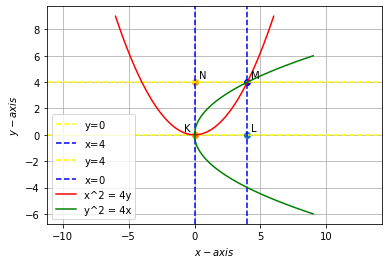
\includegraphics[width=\columnwidth]{solutions/oct/2/37/Figure/AS_5.png}
\caption{plot}
\label{2/37/fig:my_label}
\end{figure}

\begin{tabular}{ |p{2cm}||p{1.5cm}|p{1.5cm}|p{1.5cm}|p{1cm}|p{1cm}|p{1cm}| p{1cm}|p{1.5cm}|p{1.5cm}|}
 \hline
 Parabola & $\vec{V}$ & $\vec{u}$ &$f$&$\vec{q}$ & $\vec{m}$& $\mu_1$ & $\mu_2$& $\vec{POI_1}$ & $\vec{POI_2}$ \\
 \hline
 $x^2 = 4y$   & $\myvec{1 & 0 \\ 0 & 0}$    & $\myvec{0 \\ -2}$ & 0 & $\myvec{0 \\ 4}$ & $\myvec{1 \\ 0}$&4 & -4& $\myvec{4 \\ 4}$ & $\myvec{-4 \\ 4}$\\
 \hline
 $x^2 = 4y$  &   $\myvec{1 & 0 \\ 0 & 0}$ & $\myvec{0 \\ -2}$   &0 & $\myvec{0 \\ 0}$ & $\myvec{1 \\ 0}$& 0 & - & $\myvec{0 \\ 0}$&-\\
 \hline
 $y^2 = 4x$ &$\myvec{0 & 0 \\ 0 & 1}$& $\myvec{-2 \\ 0}$   &0 & $\myvec{0 \\ 4}$  & $\myvec{1 \\ 0}$& 4& - & $\myvec{4 \\ 4}$&-\\
 \hline
 $y^2 = 4x$ &$\myvec{0 & 0 \\ 0 & 1}$& $\myvec{-2 \\ 0}$    &0  & $\myvec{0 \\ 0}$  & $\myvec{1 \\ 0}$& 0& - & $\myvec{0 \\ 0}$&-\\
 
 \hline
\end{tabular}

%
\item Find the roots of the equation $5x^2  – 6x – 2 = 0 $.
\item Find the roots of $4x^2 + 3x + 5 = 0 $.
\item Find the roots of the following quadratic equations, if they exist.
\begin{enumerate}
    \item
    \begin{align}
    \begin{split}
    3x^2-5x+2&=0 \label{quad/2/23/1.0.1}
    \end{split}
    \end{align}
    \item
    \begin{align}
    \begin{split}
    x^2+4x+5&=0 \label{quad/2/23/1.0.2}
    \end{split}
    \end{align}
    \item 	$2x^2-2\sqrt{2}x+1 = 0$
\end{enumerate}
%
\solution
\begin{enumerate}

\begin{table}[!ht]
\centering
\resizebox{\columnwidth}{!}{\begin{tabular}{|c|c|c|c|} 
\hline
kind of  cake & No.of cakes & Flour& Fat\\
\hline
1st & x & 200g  &  25g \\ 
\hline
2nd& y& 100g&  50g  \\ 
\hline
Total& x+y& 5 kg=5000g&1kg=1000g \\ 
\hline
\end{tabular}}
\caption{Ingredients used in making the cake is flour and fat }
\label{opt/13/tab:table1}
\end{table}
Let the  1st kind  be $x$ and the 2nd kind be $y$  such that 
\begin{align}
x \geq 0 \\
y \geq 0 
\end{align}
According to the question,
\begin{align}
2{x} + {y} \leq 50
\\
{x} + 2{y} \leq 40
\end{align}
$\therefore$ Our problem is
\begin{align}
\max_{\vec{x}} Z &= \myvec{1& 1}\vec{x}\\
s.t. \quad \myvec{2 & 1 \\ 1& 2}\vec{x} &\preceq \myvec{50\\40} 
\end{align}
Lagrangian function is given by
\begin{equation}
\begin{aligned}
&L(\vec{x},\boldsymbol{\lambda}) \\ &= \myvec{1 & 1}\vec{x}+\lcbrak{\sbrak{\myvec{2 & 1}\vec{x}-50}} \\ &+ \sbrak{\myvec{1 & 2}\vec{x}-40}\\ &+ \sbrak{\myvec{-1 & 0}\vec{x}} +\rcbrak{\sbrak{\myvec{0 & -1}\vec{x}}}\boldsymbol{\lambda}
\end{aligned}
\end{equation}
where,
\begin{align}
\boldsymbol{\lambda} &= \myvec{\lambda_1 \\ \lambda_2 \\ \lambda_3 \\ \lambda_4 \\ \lambda_5 \\ \lambda_6}
\end{align}
Now,
\begin{align}
\nabla L(\vec{x},\boldsymbol{\lambda}) &= \myvec{1+ \myvec{2 & 1 & -1 & 0 }\boldsymbol{\lambda}\\ 1+\myvec{1 & 2 & 0 & -1}\boldsymbol{\lambda} \\ \myvec{2 & 1}\vec{x}-50\\ \myvec{1& 2}\vec{x}-40 \\  \myvec{-1 & 0}\vec{x} \\ \myvec{0 & -1}\vec{x}}
\end{align}
$\therefore$ Lagrangian matrix is given by
\begin{align}
\myvec{0 & 0 & 2 & 1& -1 & 0 \\ 0 & 0 & 1 & 2  & 0 & -1 \\ 2 & 1 & 0 & 0 & 0 & 0 \\ 1 & 2 & 0 & 0 & 0 & 0  \\ -1 & 0 & 0 & 0 & 0 & 0  \\ 0 & -1 & 0 & 0 & 0 & 0 }\myvec{\vec{x} \\ \boldsymbol{\lambda} } &= \myvec{-1 \\ -1 \\ 50\\ 4 0\\ 0 \\0 }
\end{align}
Considering $\lambda_1,\lambda_2$ as only active multiplier,
\begin{align}
\myvec{0 & 0 & 2 & 1 \\ 0 & 0 & 1 & 2 \\ 2 & 1 & 0 & 0 \\ 1 & 2 & 0 & 0}\myvec{\vec{x}\\ \boldsymbol{\lambda}} &= \myvec{-1 \\ -1 \\ 5 0\\ 40}
\end{align}
resulting in,
\begin{align}
\myvec{\vec{x} \\ \boldsymbol{\lambda}} &= \myvec{0 & 0 & 2 & 1 \\ 0 & 0 & 1 & 2 \\ 2 & 1 & 0 & 0 \\ 1& 2 & 0 & 0}^{-1}\myvec{-1 \\ -1 \\ 50 \\ 40}
\\
\implies   \myvec{\vec{x} \\ \boldsymbol{\lambda}} &= \myvec{0 & 0 & \frac{2}{3} & \frac{-1}{3} \\ 0 & 0 & \frac{-1}{3} & \frac{2}{3} \\ \frac{2}{3} & \frac{-1}{3} & 0 & 0 \\ \frac{-1}{3} & \frac{2}{3} & 0 & 0}\myvec{-1 \\ -1 \\ 50 \\ 40}
\\
\implies \myvec{\vec{x} \\ \boldsymbol{\lambda}} &= \myvec{20 \\ 10 \\ -0.3 \\ -0.3 }
\end{align}
$\because \boldsymbol{\lambda}=\myvec{-0.3 \\ -0.3} \succ \vec{0} $
\\
$\therefore$ Optimal solution is given by
\begin{align}
    \vec{x} &= \myvec{20\\10} \\
    Z &= \myvec{1& 1}\vec{x} \\
    &= \myvec{1 & 1}\myvec{20 \\ 10} \\
    &= 60
\end{align}
By using cvxpy in python ,
\begin{align}
    \vec{x}=\myvec{20\\10}\\
    Z = 60
\end{align}
Hence No.of cakes \boxed{x=20} 1st kind and  .of cakes \boxed{y=10} 2nd kind should be used to maximum No. of cakes \boxed{Z=60}.  This is
verified in Fig. \ref{opt/13/fig: Graphical Solution}.	
%
\begin{figure}[!ht]
\centering
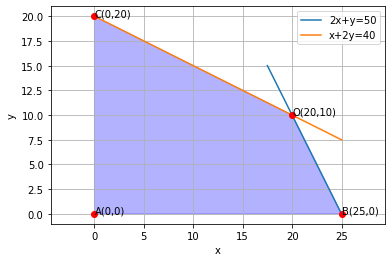
\includegraphics[width=\columnwidth]{solutions/su2021/2/13/Figure9.png}
\caption{Graphical Solution}
\label{opt/13/fig: Graphical Solution}	
\end{figure}

\end{enumerate}

\item Solve $x^2+ 2 = 0 $.
\\
\solution
\documentclass[journal,12pt,twocolumn]{IEEEtran}

\usepackage{setspace}
\usepackage{gensymb}

\singlespacing


\usepackage[cmex10]{amsmath}

\usepackage{amsthm}

\usepackage{mathrsfs}
\usepackage{txfonts}
\usepackage{stfloats}
\usepackage{bm}
\usepackage{cite}
\usepackage{cases}
\usepackage{subfig}

\usepackage{longtable}
\usepackage{multirow}

\usepackage{enumitem}
\usepackage{mathtools}
\usepackage{steinmetz}
\usepackage{tikz}
\usepackage{circuitikz}
\usepackage{verbatim}
\usepackage{tfrupee}
\usepackage[breaklinks=true]{hyperref}
\usepackage{graphicx}
\usepackage{tkz-euclide}
\usepackage{float}

\usetikzlibrary{calc,math}
\usepackage{listings}
    \usepackage{color}                                            %%
    \usepackage{array}                                            %%
    \usepackage{longtable}                                        %%
    \usepackage{calc}                                             %%
    \usepackage{multirow}                                         %%
    \usepackage{hhline}                                           %%
    \usepackage{ifthen}                                           %%
    \usepackage{lscape}     
\usepackage{multicol}
\usepackage{chngcntr}

\DeclareMathOperator*{\Res}{Res}

\renewcommand\thesection{\arabic{section}}
\renewcommand\thesubsection{\thesection.\arabic{subsection}}
\renewcommand\thesubsubsection{\thesubsection.\arabic{subsubsection}}

\renewcommand\thesectiondis{\arabic{section}}
\renewcommand\thesubsectiondis{\thesectiondis.\arabic{subsection}}
\renewcommand\thesubsubsectiondis{\thesubsectiondis.\arabic{subsubsection}}


\hyphenation{op-tical net-works semi-conduc-tor}
\def\inputGnumericTable{}                                 %%

\lstset{
%language=C,
frame=single, 
breaklines=true,
columns=fullflexible
}
\begin{document}


\newtheorem{theorem}{Theorem}[section]
\newtheorem{problem}{Problem}
\newtheorem{proposition}{Proposition}[section]
\newtheorem{lemma}{Lemma}[section]
\newtheorem{corollary}[theorem]{Corollary}
\newtheorem{example}{Example}[section]
\newtheorem{definition}[problem]{Definition}

\newcommand{\BEQA}{\begin{eqnarray}}
\newcommand{\EEQA}{\end{eqnarray}}
\newcommand{\define}{\stackrel{\triangle}{=}}
\bibliographystyle{IEEEtran}
\providecommand{\mbf}{\mathbf}
\providecommand{\pr}[1]{\ensuremath{\Pr\left(#1\right)}}
\providecommand{\qfunc}[1]{\ensuremath{Q\left(#1\right)}}
\providecommand{\sbrak}[1]{\ensuremath{{}\left[#1\right]}}
\providecommand{\lsbrak}[1]{\ensuremath{{}\left[#1\right.}}
\providecommand{\rsbrak}[1]{\ensuremath{{}\left.#1\right]}}
\providecommand{\brak}[1]{\ensuremath{\left(#1\right)}}
\providecommand{\lbrak}[1]{\ensuremath{\left(#1\right.}}
\providecommand{\rbrak}[1]{\ensuremath{\left.#1\right)}}
\providecommand{\cbrak}[1]{\ensuremath{\left\{#1\right\}}}
\providecommand{\lcbrak}[1]{\ensuremath{\left\{#1\right.}}
\providecommand{\rcbrak}[1]{\ensuremath{\left.#1\right\}}}
\theoremstyle{remark}
\newtheorem{rem}{Remark}
\newcommand{\sgn}{\mathop{\mathrm{sgn}}}
\providecommand{\abs}[1]{\left\vert#1\right\vert}
\providecommand{\res}[1]{\Res\displaylimits_{#1}} 
\providecommand{\norm}[1]{\left\lVert#1\right\rVert}
%\providecommand{\norm}[1]{\lVert#1\rVert}
\providecommand{\mtx}[1]{\mathbf{#1}}
\providecommand{\mean}[1]{E\left[ #1 \right]}
\providecommand{\fourier}{\overset{\mathcal{F}}{ \rightleftharpoons}}
%\providecommand{\hilbert}{\overset{\mathcal{H}}{ \rightleftharpoons}}
\providecommand{\system}{\overset{\mathcal{H}}{ \longleftrightarrow}}
	%\newcommand{\solution}[2]{\textbf{Solution:}{#1}}
\newcommand{\solution}{\noindent \textbf{Solution: }}
\newcommand{\cosec}{\,\text{cosec}\,}
\providecommand{\dec}[2]{\ensuremath{\overset{#1}{\underset{#2}{\gtrless}}}}
\newcommand{\myvec}[1]{\ensuremath{\begin{pmatrix}#1\end{pmatrix}}}
\newcommand{\mydet}[1]{\ensuremath{\begin{vmatrix}#1\end{vmatrix}}}
\numberwithin{equation}{subsection}
\makeatletter
\@addtoreset{figure}{problem}
\makeatother
\let\StandardTheFigure\thefigure
\let\vec\mathbf
\renewcommand{\thefigure}{\theproblem}
\def\putbox#1#2#3{\makebox[0in][l]{\makebox[#1][l]{}\raisebox{\baselineskip}[0in][0in]{\raisebox{#2}[0in][0in]{#3}}}}
     \def\rightbox#1{\makebox[0in][r]{#1}}
     \def\centbox#1{\makebox[0in]{#1}}
     \def\topbox#1{\raisebox{-\baselineskip}[0in][0in]{#1}}
     \def\midbox#1{\raisebox{-0.5\baselineskip}[0in][0in]{#1}}
\vspace{3cm}
\title{Assignment 5}
\author{K.A. Raja Babu}
\maketitle
\newpage
\bigskip
\renewcommand{\thefigure}{\theenumi}
\renewcommand{\thetable}{\theenumi}
Download all python codes from 
\begin{lstlisting}
https://github.com/ka-raja-babu/Matrix-Theory/tree/main/Assignment5/Codes
\end{lstlisting}
%
and latex-tikz codes from 
%
\begin{lstlisting}
https://github.com/ka-raja-babu/Matrix-Theory/tree/main/Assignment5
\end{lstlisting}
%
\section{Question No. 2.1}
Find the equation of the circle with radius 5 whose centre lies on x-axis and passes through the point \myvec{2\\3} .
%
\section{Solution}
Let $\vec{O}$ be the centre and $r$ be the radius of the given circle.
\\
$\therefore$
\begin{align}
\vec{O} &= \myvec{p\\0}
\\
r &= 5
\end{align}

General equation of a circle is given by 
\begin{align}
\vec{x}^T\vec{x} - 2\vec{O}^T\vec{x} + \norm{\vec{O}}^2 -r^2 = 0
\end{align}

$\therefore$
The equation of the given circle is
\begin{align}
\vec{x}^T\vec{x} - 2\myvec{p & 0}\vec{x} + p^2 - 25 = 0
\end{align}

$\because$
Point $\vec{A}$=\myvec{2\\3} lies on this equation and satisfies it.
\\
$\therefore$
\begin{align}
\myvec{2 & 3}\myvec{2\\3} - 2\myvec{p & 0}\myvec{2\\3} + p^2 -25 &=0
\\
\implies 13 - 4p + p^2 -25 &=0
\\
\implies p^2 - 4p - 12 &=0
\\
\implies p &=6 
\\
\text{or} , p &=-2
\end{align}

Hence,the equation of the circle can be written as
\begin{align}
\vec{x}^T\vec{x} - 2\myvec{6 & 0}\vec{x} + 11 &= 0 \label{eq:1}
\\
\text{or}, \vec{x}^T\vec{x} - 2\myvec{-2 & 0}\vec{x} - 21 &= 0 \label{eq:2}
\end{align}

Plot of the equations \eqref{eq:1} and \eqref{eq:2}

\numberwithin{figure}{section}
\begin{figure}[!ht]
\centering
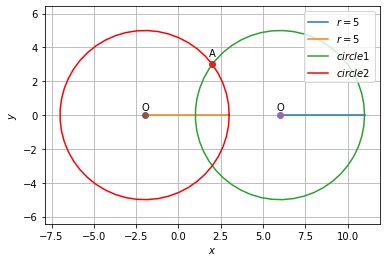
\includegraphics[width=\columnwidth]{Figure5}
\caption{Circles with centres (6,0) and (-2,0) respectively }
\label{fig:circle}	
\end{figure}

\end{document}

\item Solve $x^2+ x+1 = 0 $.
\item Solve $\sqrt{5}x^2+ x+\sqrt{5} = 0 $.
%
\item Find the coordinates of the focus, axis, the equation of the directrix and latus rectum of the parabola $y^2 = 8x$.
%

\item Find the equation of the parabola which is symmetric about the y-axis, and passes through the point \myvec{2\\–3}.
\item Find the coordinates of the foci, the vertices, the length of major axis, the minor axis, the eccentricity and the latus rectum of the ellipse 
%
\begin{align}
\vec{x}^T\myvec{\frac{1}{25} & 0 \\ 0 & \frac{1}{9}}\vec{x} = 1
\end{align}
%
\item Find the coordinates of the foci, the vertices, the lengths of major and minor axes and the eccentricity of the ellipse 
%
\begin{align}
\vec{x}^T\myvec{9 & 0 \\ 0 & 4}\vec{x} = 36
\end{align}
%
\item Find the equation of the ellipse whose vertices are $\myvec{\pm 13\\ 0}$ and foci are $\myvec{\pm 5\\ 0}$.
%
\item Find the equation of the ellipse, whose length of the major axis is 20 and foci are $\myvec{0\\ \pm 5}$
%

\item Find the equation of the hyperbola with  vertices $\myvec{0 \\ \pm \frac{\sqrt{11}}{2}}$, foci $\myvec{ 0\\ \pm 3}$
\item Find the equation of the hyperbola with   foci $\myvec{ 0\\ \pm 12}$ and length of latus rectum 36.
%

\item Find the roots of the following equations:
\begin{enumerate}
\item  $x + \frac{1}{x} = 3, x \ne =0 $
\item  $ \frac{1}{x} + \frac{1}{x-2}=3, x\ne =0, 2 $
\end{enumerate}
%
\solution
\begin{enumerate}
\item 
\begin{table}[!ht]
\centering
\resizebox{\columnwidth}{!}{\begin{tabular}{|c|c|c|c|} 
\hline
kind of  cake & No.of cakes & Flour& Fat\\
\hline
1st & x & 200g  &  25g \\ 
\hline
2nd& y& 100g&  50g  \\ 
\hline
Total& x+y& 5 kg=5000g&1kg=1000g \\ 
\hline
\end{tabular}}
\caption{Ingredients used in making the cake is flour and fat }
\label{opt/13/tab:table1}
\end{table}
Let the  1st kind  be $x$ and the 2nd kind be $y$  such that 
\begin{align}
x \geq 0 \\
y \geq 0 
\end{align}
According to the question,
\begin{align}
2{x} + {y} \leq 50
\\
{x} + 2{y} \leq 40
\end{align}
$\therefore$ Our problem is
\begin{align}
\max_{\vec{x}} Z &= \myvec{1& 1}\vec{x}\\
s.t. \quad \myvec{2 & 1 \\ 1& 2}\vec{x} &\preceq \myvec{50\\40} 
\end{align}
Lagrangian function is given by
\begin{equation}
\begin{aligned}
&L(\vec{x},\boldsymbol{\lambda}) \\ &= \myvec{1 & 1}\vec{x}+\lcbrak{\sbrak{\myvec{2 & 1}\vec{x}-50}} \\ &+ \sbrak{\myvec{1 & 2}\vec{x}-40}\\ &+ \sbrak{\myvec{-1 & 0}\vec{x}} +\rcbrak{\sbrak{\myvec{0 & -1}\vec{x}}}\boldsymbol{\lambda}
\end{aligned}
\end{equation}
where,
\begin{align}
\boldsymbol{\lambda} &= \myvec{\lambda_1 \\ \lambda_2 \\ \lambda_3 \\ \lambda_4 \\ \lambda_5 \\ \lambda_6}
\end{align}
Now,
\begin{align}
\nabla L(\vec{x},\boldsymbol{\lambda}) &= \myvec{1+ \myvec{2 & 1 & -1 & 0 }\boldsymbol{\lambda}\\ 1+\myvec{1 & 2 & 0 & -1}\boldsymbol{\lambda} \\ \myvec{2 & 1}\vec{x}-50\\ \myvec{1& 2}\vec{x}-40 \\  \myvec{-1 & 0}\vec{x} \\ \myvec{0 & -1}\vec{x}}
\end{align}
$\therefore$ Lagrangian matrix is given by
\begin{align}
\myvec{0 & 0 & 2 & 1& -1 & 0 \\ 0 & 0 & 1 & 2  & 0 & -1 \\ 2 & 1 & 0 & 0 & 0 & 0 \\ 1 & 2 & 0 & 0 & 0 & 0  \\ -1 & 0 & 0 & 0 & 0 & 0  \\ 0 & -1 & 0 & 0 & 0 & 0 }\myvec{\vec{x} \\ \boldsymbol{\lambda} } &= \myvec{-1 \\ -1 \\ 50\\ 4 0\\ 0 \\0 }
\end{align}
Considering $\lambda_1,\lambda_2$ as only active multiplier,
\begin{align}
\myvec{0 & 0 & 2 & 1 \\ 0 & 0 & 1 & 2 \\ 2 & 1 & 0 & 0 \\ 1 & 2 & 0 & 0}\myvec{\vec{x}\\ \boldsymbol{\lambda}} &= \myvec{-1 \\ -1 \\ 5 0\\ 40}
\end{align}
resulting in,
\begin{align}
\myvec{\vec{x} \\ \boldsymbol{\lambda}} &= \myvec{0 & 0 & 2 & 1 \\ 0 & 0 & 1 & 2 \\ 2 & 1 & 0 & 0 \\ 1& 2 & 0 & 0}^{-1}\myvec{-1 \\ -1 \\ 50 \\ 40}
\\
\implies   \myvec{\vec{x} \\ \boldsymbol{\lambda}} &= \myvec{0 & 0 & \frac{2}{3} & \frac{-1}{3} \\ 0 & 0 & \frac{-1}{3} & \frac{2}{3} \\ \frac{2}{3} & \frac{-1}{3} & 0 & 0 \\ \frac{-1}{3} & \frac{2}{3} & 0 & 0}\myvec{-1 \\ -1 \\ 50 \\ 40}
\\
\implies \myvec{\vec{x} \\ \boldsymbol{\lambda}} &= \myvec{20 \\ 10 \\ -0.3 \\ -0.3 }
\end{align}
$\because \boldsymbol{\lambda}=\myvec{-0.3 \\ -0.3} \succ \vec{0} $
\\
$\therefore$ Optimal solution is given by
\begin{align}
    \vec{x} &= \myvec{20\\10} \\
    Z &= \myvec{1& 1}\vec{x} \\
    &= \myvec{1 & 1}\myvec{20 \\ 10} \\
    &= 60
\end{align}
By using cvxpy in python ,
\begin{align}
    \vec{x}=\myvec{20\\10}\\
    Z = 60
\end{align}
Hence No.of cakes \boxed{x=20} 1st kind and  .of cakes \boxed{y=10} 2nd kind should be used to maximum No. of cakes \boxed{Z=60}.  This is
verified in Fig. \ref{opt/13/fig: Graphical Solution}.	
%
\begin{figure}[!ht]
\centering
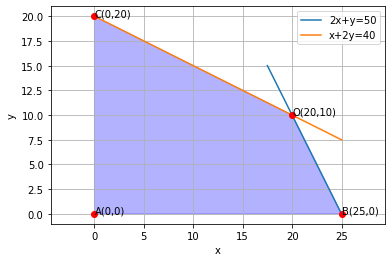
\includegraphics[width=\columnwidth]{solutions/su2021/2/13/Figure9.png}
\caption{Graphical Solution}
\label{opt/13/fig: Graphical Solution}	
\end{figure}

\end{enumerate}


\item Find points on the curve 
$
\vec{x}^T\myvec{\frac{1}{4} & 0 \\ 0 & \frac{1}{25}}\vec{x} = 1
$
at which the tangents are 
\begin{enumerate}
\item parallel to x-axis
\item parallel to y-axis
\end{enumerate}
 
\item Find the area enclosed by the ellipse
$
\vec{x}^T\myvec{\frac{1}{a^2} & 0 \\ 0 & \frac{1}{b^2}}\vec{x} = 1
$
%
\item Find the area of the region bounded by the curve $y = x^2$
and the line $y = 4$.
%
\item Find the area bounded by the ellipse
$
\vec{x}^T\myvec{\frac{1}{a^2} & 0 \\ 0 & \frac{1}{b^2}}\vec{x} = 1
$
and $x = ae$, where, $b^2 = a^2 (1 – e^2 )$ and $e < 1$.
%
\item Prove that the curves $y^2 = 4x$ and $x^2 = 4y$ divide the area of the square bounded by $x = 0, x = 4, y =4$ and $y = 0$ into three equal parts.
%
\item Find the area of the region
\begin{align}
\cbrak{\brak{x,y} = 0\le y\le x^2+1, 0\le y \le x+1, 0 \le x \le 2}
\end{align}

%\item Find the shortest distance of the point $\myvec{0\\c}$ from the parabola $y = x^2$, where $\frac{1}{2} \le c \le 5$.
%
%\item An apache helicopter of enemy is flying along the curve given by $y = x^2+7$.  A soldier, placed at \myvec{3\\7}, wants to shoot down the helicopter when it is nearest to him.  Find  the nearest distance.
%
\item Examine whether the function $f$ given by $f(x) = x^2$ is continuous at $x = 0$.
%
\item Discuss the continuity of the function $f$ defined by 
%
\begin{align}
f(x)  = 
\begin{cases}
x & x \ge 0
\\
x^2 & x < 0
\end{cases}
\end{align}
%
\item Verify Rolle's theorem for the function $y = x^2+2, a = -2$ and $b = 2$.
\item Verify Mean Value Theorem for the function $f(x) = x^2$ in the interval $\sbrak{2,-4}$.
%\end{align}
\item Find the derivative of $f(x) = x^2$.
\item Find the derivative of $ x^2 - 2$ at $x = 10$.
\item Find the derivative of $ \brak{x-1} \brak{x-2}$.
%
%
\item Find 
\begin{align}
\int_{0}^{2} \brak{x^2+1}\,dx
\end{align}
%
as a limit of a sum.
\item Evaluate the following integral:
%
\begin{align}
\int_{2}^{3}x^2 \,dx
\end{align}
%
\item Form the differntial equation representing the family of ellipses having foci on x-axis and cenre at the origin.
%
\item Form the differntial equation representing the family of parabolas having vertex at origin and axis along positive direction of x-axis.
\item Form a differntial equation representing the following family of curves
%
\begin{align}
y^2 = a\brak{b^2-x^2}
\end{align}
%
\item  A cricket ball is thrown at a speed of 28 $m s^{-1}$
in a direction 30$\degree$ above
the horizontal. Calculate 
\begin{enumerate}
\item  the maximum height, 
\item  the time taken by the ball to return to the same level, and 
\item  the distance from the thrower to the point where the ball returns to the same level.
\end{enumerate}
\item Find the roots of the equation  $2x^2– 5x + 3 = 0$ .
\item Find the value of  the following polynomial at the indicated value of variables 
\begin{align}
p(x) = 5x^2– 3x + 7 \text{  at } x = 1.
\end{align}
%\end{enumerate}
